        \clearpage
        \begin{figure*}[ht]
            \pdfbookmark[2]{ID 06}{figure_id_06}
        	\centering
            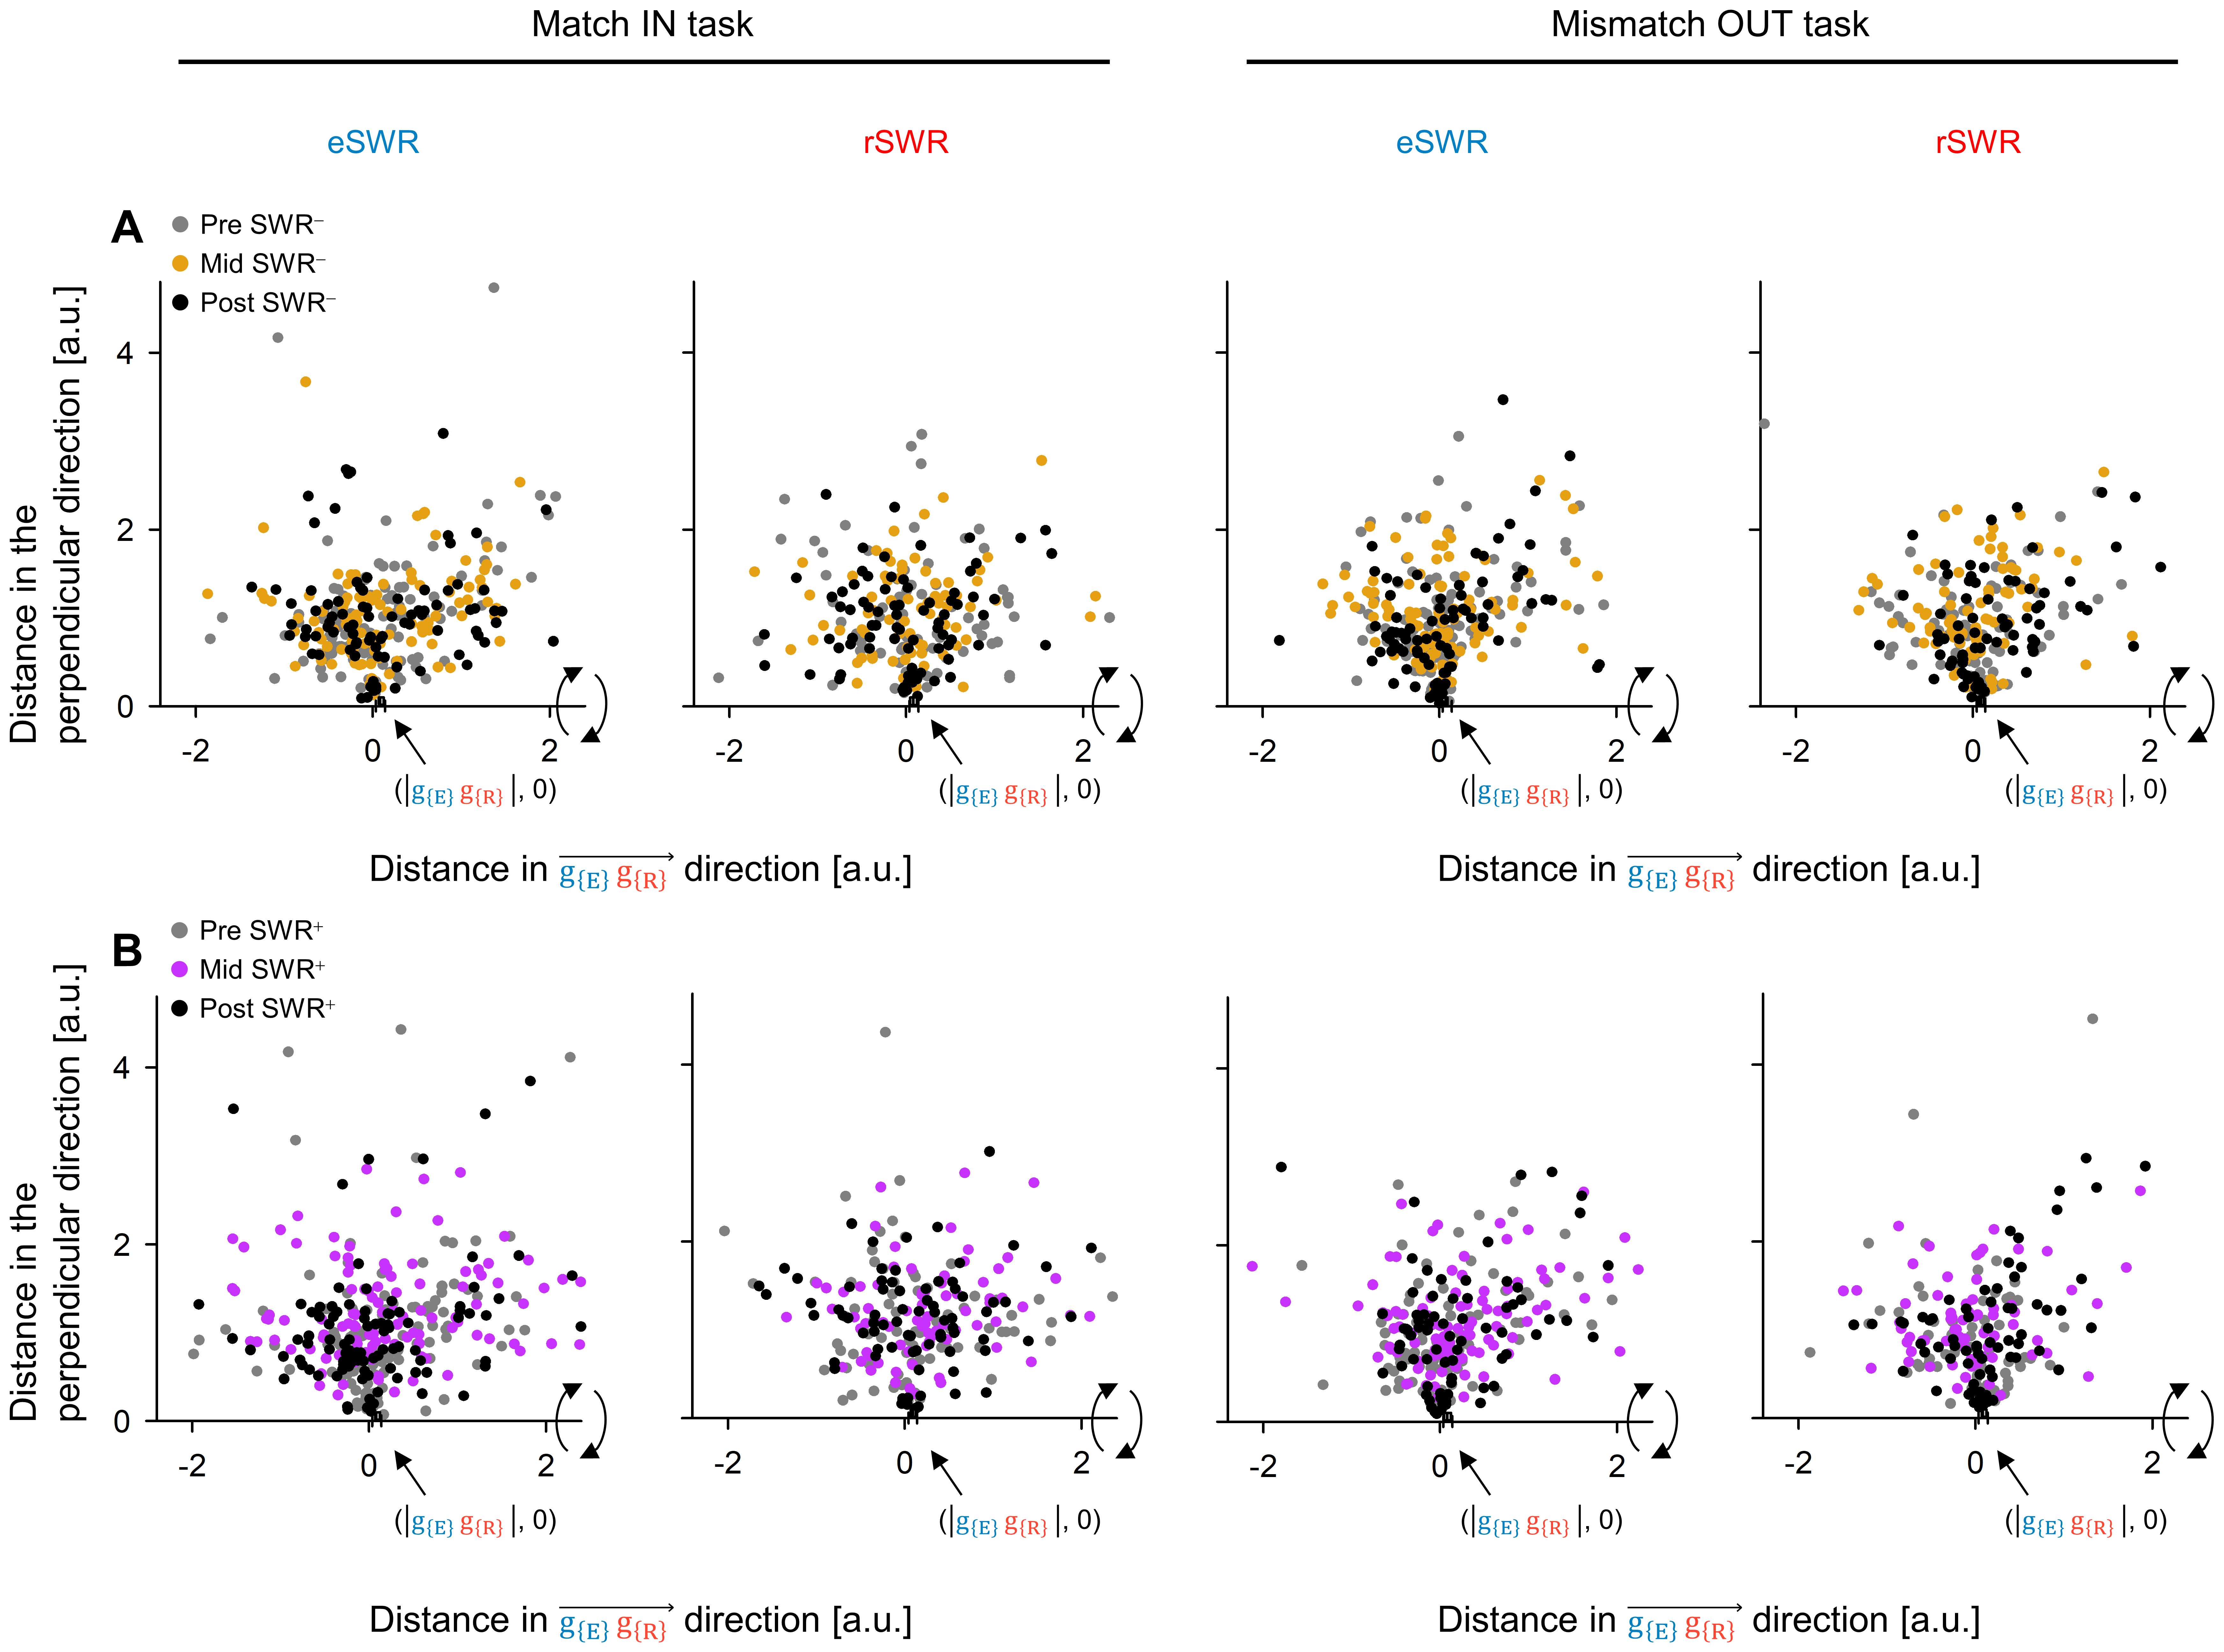
\includegraphics[width=1\textwidth]{./src/figures/.png/Figure_ID_06.png}
        	\caption{\textbf{
Visualization of neural trajectory during SWR in two-dimensional spaces
}
\smallskip
\\
Panels show hippocampal neural trajectories during SWR, which were projected into two-dimensional spaces. \textbf{\textit{A.}} Hippocampal neural trajectories during pre- (\textit{gray}), mid- (\textit{yellow}), and post-SWR$^-$ (\textit{black}). \textbf{\textit{B.}} The equivalents for SWR$^+$, instead of SWR$^-$. The $\lVert \mathrm{g_{E}g_{R}} \rVert$ varied across sessions. The projection was applied as follows. First, linear transformation was applied in the way that $\mathrm{g_{E}}$ was placed at the origin $O$ (0, 0), and $\mathrm{g_{R}}$ at ($\lVert \mathrm{g_{E}g_{R}} \rVert$, 0). Moreover, point cloud was rotated around the $\mathrm{g_{E}g_{R}}$ axis (= x axis) to fit in two-dimensional spaces. Thus, in these two-dimensional spaces, both the distances from $O$ and angles between the $\mathrm{g_{E}g_{R}}$ axis are preserved from the original three dimensional spaces. Abbreviations: SWR, sharp-wave ripple events; eSWR, SWR during the encoding phase; rSWR, SWR during the retrieval phase, SWR$^+$, SWR event; SWR$^-$ control events for SWR$^+$; pre-SWR, mid-SWR, or post-SWR, the time interval from $-800$ to $-250$ ms, from $-250$ to $+250$ ms, or from $+250$ to $+800$ ms from the center of SWR. 
}
% width=1\textwidth
        	\label{fig:06}
        \end{figure*}
